\documentclass{school-22.101-notes}
\date{November 28, 2011}

\begin{document}
\maketitle

\lecture{Neutron Interactions}
Neutrons interact primarily with the nucleus of an atom. Neutron interactions can take place at \textit{any energy}, so we care about the energy variation of interaction cross-section (interacting probability). Neutrons in a nuclear reactor have energies between $10^{-3} \sim 10^7$ eV (Figure~\ref{neutron-energy}).  
\begin{figure}[ht]
    \centering
    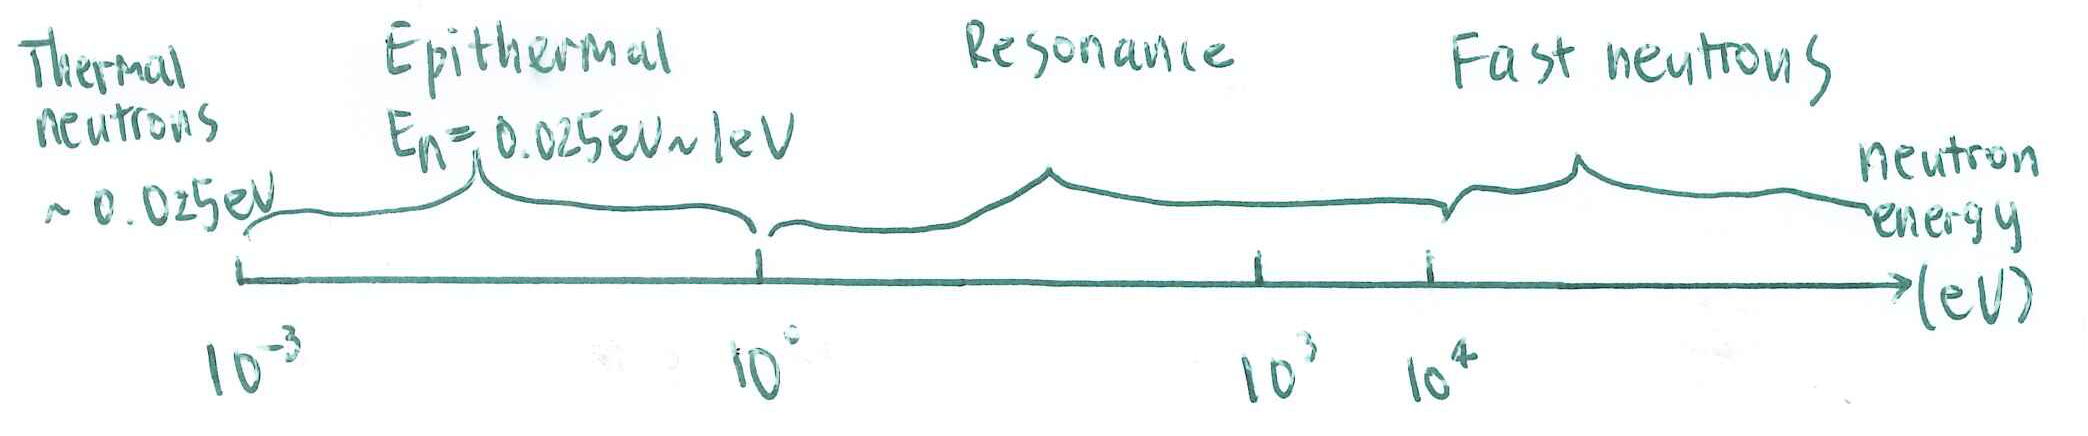
\includegraphics[width=5in]{images/ni/neutron-energy.png}
    \caption{Neutron Energy Range\label{neutron-energy}}
\end{figure}
Within this range, important neutron interactions are: 
\begin{enumerate}
\item $(n,n)$ Elastic Scattering: 
    \begin{itemize}
    \item* Potential Scattering (billard-ball like collision);
    \item Resonance Scattering (compound nucleus formation and decay);
    \end{itemize}
\item* $(n,n^{\prime})$ Inelastic Scattering (excitation of nuclear levels);
\item $(n, \gamma)$ Radiative Capture (get hit by a neutron, release $\gamma$ ray);
\item $(n, p), (n,\alpha), \cdots$ Charged Particle Emission;
\item $(n, f)$ fission.     
\end{enumerate}
We will cover the two entries with * in this lecture; the rest of the topics will be covered by introducing the `compound nucleus' model (which is one model to explain them; not necessarily the only one). 


There are three major tropics in this chapter: 
\begin{enumerate}
\item Basics: kinemetics. 
\item Elastic scattering: distribution. 
\item Cross sections: neutron reactions. 
\end{enumerate}


A brief history: 
\begin{itemize}
\item Discovery of neutrons: Chadwick 1932. 
\item Discovery of fission: Hahn 1938. 
\item Chicago Pile 1. 
\item Bombs. 
\end{itemize}

Prof. Yip on 11/19/12: arrive at $Q$ equation (15.5 in SY3), and discuss two cases: 
\begin{itemize}
\item $Q = 0$ for elastic scattering. If $E_1 = E_3$, then forward scattering, 
\item $Q < 0$ for inelastic scattering (endothermal reaction, energy has to be inputed, implying that there is a nuclear excitation). The center of mass is what requires the energy `tax': $E_{\mathrm{threshold}} \sim E^* \left( 1 + \frac{1}{A} \right)$.   Know how to draw and derive the velocity relations. Meyerham's Fig. 15.5 is missing a negative sign. Know
  \eqn{ E_3 = \frac{1}{2} E_1 \left[ (1+ \alpha) + (1 - \alpha) \cos \theta_C \right] }
  which relates $E_3$ with the scattering angle; this is the reason we went to CMCS because that relation in the lab system is very complicated. 
\end{itemize}

\topic{Scattering Kinematics, Lab CS}
\subtopic{Q-equation: Energetics of Scattering} 
\begin{figure}[ht]
    \centering
    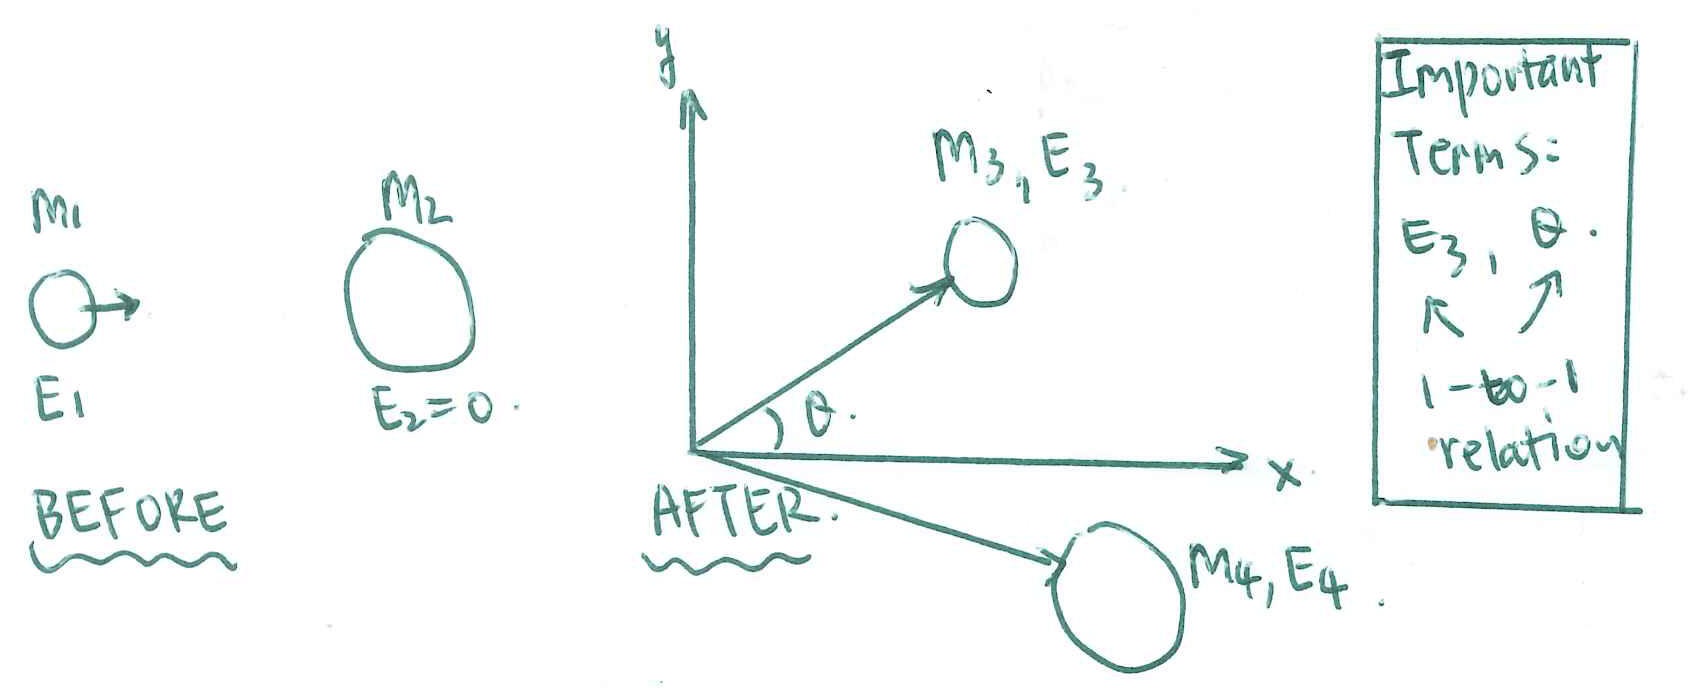
\includegraphics[width=4in]{images/ni/setup-lab.png}
    \caption{Setup of Scattering in Lab Frame\label{setup-lab}}
\end{figure}
Figure~\ref{setup-lab} demonstrates the set-up of the scattering collision. The ultimate goal is to relate $T_3$ and $\theta$, and to find the energy and angular distribution of elastically scattered neutrons. 
We want to keep it general for now (elastic, inelastic). Apply conservation of energy and momentum: 
\begin{align}
Q &= \Sum m_i c^2 - \Sum m_f c^2 = \Sum T_f - \Sum T_i \\
(m_1 c^2 + E_1 ) + m_2 c^2 &= m_3 c^3 + E_3 + m_4 c^2 + E_4 \\
\vecp_1 &= \vecp_3 + \vecp_4 \\
\vecp_4^2 &= (\vecp_1 - \vecp_3)^2 \\
T_4 &= \frac{p_1^2 + p_3^2 - 2 p_1 p_3 \cos \theta }{2 m_4} \\
Q &= (m_1 + m_2 - m_3 - m_4) c^2 = T_3 + T_4 - T_1 \\
&= T_3  - T_1 + \frac{2 m_1 T_1}{2 m_4} + \frac{2 m_3 T_3}{2 m_4} - \frac{2}{2m_4} \sqrt{2 m_1 T_1 2 m_3 T_3} \cos \theta \\
&= T_3 \left( 1 + \frac{m_3}{m_4} \right) - T_1 \left( 1 - \frac{m_3}{m_4} \right) - \frac{2}{m_4} \sqrt{m_1 T_1 m_3 T_1} \cos \theta \label{T3-to-theta}
\end{align}
Interpretation: 
\begin{itemize}
\item Energy values, like Q, are independent of coordinate systems. 
\item Eq.~\ref{T3-to-theta} relates $T_3$ to $\theta$ in a one-to-one fashion. We have two equations, three unknowns, so we can write one as another.
\item Typically, we are given $T_1, Q$, masses, and being asked to find $T_3$ in terms of $\cos \theta$. We solve Eq.~\ref{T3-to-theta} by solving a quadratic equation. That is, Q determines $T_3$.
\item Elastic Scattering $\Rightarrow Q=0$ (energy lost by neutrons is energy gained by the recoiling target nucleus); Inelastic Scattering $\Rightarrow Q < 0$ (energy lost by neutrons is larger than energy gained by recoiling nucleus). 
\end{itemize}

\subtopic{Elastic Scattering}
Elastic scattering is the prime way fast neutrons lose energies. $m_1 = m_3 = m_n, m_2 = m_4 = m_A \approx A m_n$. 
\begin{align}
0 &= T_3 \left( 1 + \frac{1}{A} \right)  - T_1 \left( 1 - \frac{1}{A} \right) - \frac{2}{A} \sqrt{ T_1 T_3} \cos \theta \\
&\begin{dcases*}
T_3^{max} = T_1 &  $\theta = 0$,  Perfect forward scattering \\
T_3^{min} = \left( \frac{A-1}{A+1} \right)^2 T_1 = \alpha T_1 & $\theta = \pi$, Perfect backward scattering 
\end{dcases*}
\end{align}

\subtopic{Inelastic Scattering}
Inelastic Scattering $\Rightarrow Q < 0$ (energy lost by neutrons is larger than energy gained by recoiling nucleus, neutron excites the target nucleus, target nucleus gain energy through the KE of neutron, Figure~\ref{inelastic-energy}). 
\begin{figure}
    \centering
    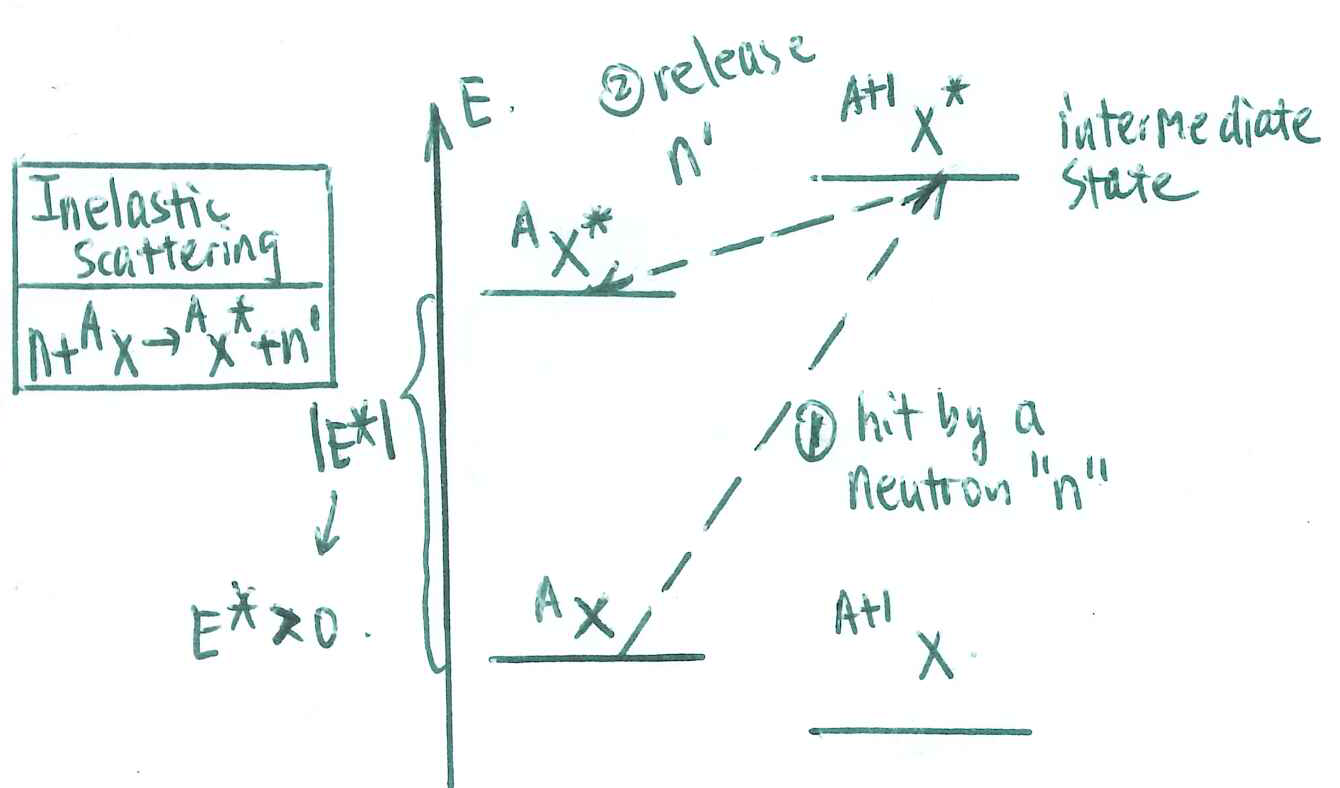
\includegraphics[width=4in]{images/ni/inelastic-energy.png}
    \caption{Energy Levels for Inelastic Scattering\label{inelastic-energy}}
\end{figure}
\begin{align}
M^* c^2 - M c^2 &= E^* > 0  & M^* &= M + \frac{E^*}{c^2} \label{M*}
\end{align}
Eq.\ref{M*} means that the excited state energy is a result from the ground state energy plus the incoming neutron's KE. The minimum KE of neutron required to induce inelastic scattering, $T_1^{min}$, corresponds to $T_3 = 0$. Plug it back into the general expression, we get 
\begin{align}
Q &= - E^* = -T_1^{min} \left( 1 - \frac{1}{A} \right) & T_1^{min} &= E^* \frac{A}{A-1} > E^* 
\end{align}
\textcolor{blue}{Minimum KE of neutron, $T_1^{min}$, is always greater than $E^*$!!!}

\topic{Scattering Kinematics, CMCS}
\begin{figure}
    \centering
    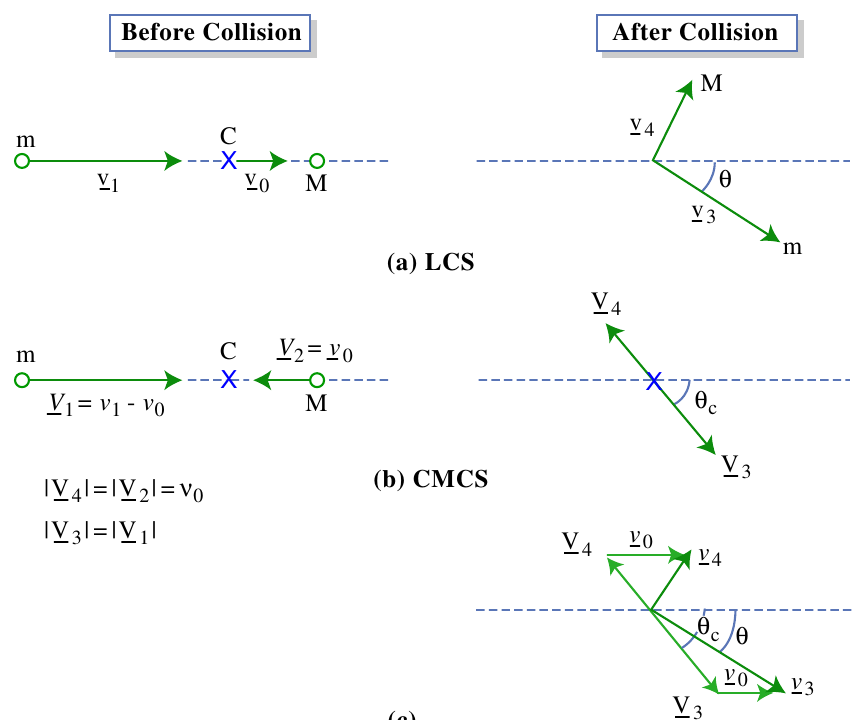
\includegraphics[width=4in]{images/ni/setup-CofM.png}
    \caption{Setup of Scattering in Center of Mass Coordinate System\label{setup-CofM}}
\end{figure}
If we consider $\vecv_1, \vecv_2, \vecv_3, \vecv_4$ as the velocities in the Lab coordinate system, $\vecV_1, \vecV_2, \vecV_3, \vecV_4$ are the velocities in the center of mass coordinate system, with $\vecv_0$ being the velocity of the center of the mass, $\theta_c$ being the new angle as in Figure~\ref{setup-CofM}. 

Conservation of energy and momentum tell us: 
\begin{align}
|\vecV_3| &= |\vecV_1| & |\vecV_4| &= |\vecV_2| = |\vecv_0| 
\end{align}
Then the Q-equation (energetics of scattering) is: 
\begin{align}
\frac{1}{2m} \vecv_3^2 &= \frac{1}{2m} \left( \vecv_3 + \vecv_0 \right)^2 = \frac{1}{2m} \left( v_3^2 + v_0^2 + 2 v_3 v_0 \cos \theta_c \right) \\
v_1 m &= v_0 (M+m) \Rightarrow v_0 = v_1 \frac{m}{M+m} = v_1 \frac{1}{A+1} \\
V_3 m &= V_4 M = v_0 M = v_1 \frac{M}{m+M} \Rightarrow V_3 = v_1 \frac{A}{A+1} \\
\Rightarrow T_3 &= \frac{1}{2} T_1 \left[ (\alpha+1 ) + (1-\alpha) \cos \theta_C \right], \fsp \alpha = \left( \frac{A-1}{A+1} \right)^2 \label{T3-to-thetaC} \\
&\begin{dcases*}
T_3^{max} = T_1 &  $\theta_C = 0$,  Perfect forward scattering \\
T_3^{min} = \alpha T_1 & $\theta_C = \pi$, Perfect backward scattering 
\end{dcases*}\\
\cos \theta &= \frac{1 + A \cos \theta_C}{\sqrt{A^2 + 1 + 2A \cos \theta_C}} \label{theta-to-thetaC}
\end{align}
Notice Eq.~\ref{T3-to-thetaC} is the important equation that relate $T_3$ to $\theta_C$ in a one-to-one fashion. The value of the minimum and maximum $T_3$ are the same as in the lab coordinate system. Eq.\ref{theta-to-thetaC} relates $\theta$ to $\theta_C$ in a one-to-one fashion. 

\topic{Energy Dependency of Elastic Scattering Cross-Sections $\sigma_S(E)$}
Three Assumptions:
\begin{enumerate}
\item Elastic scattering;
\item Target at rest;
\item S-wave scattering, that is, $E \le 10$ keV, isotropic in Center-of-Mass frame.
\end{enumerate}
The goal is to find $P(T_1 \to T_3) \dT_3 = P(\Omega_C) \dOmega_C = P(\theta_C) \dtheta_C.$ We start from the right to left. Consider $P(\Omega_C) \dOmega_C$ as the probability of neutron getting into $\dOmega_C$ about $\Omega_C$. Below, notice $P(\Omega_C) = \frac{1}{4 \pi}$ for S-wave scattering. 
\begin{align}
\int_0^{2 \pi} \dOmega_C \int_0^{\pi} \sin \theta_C P(\Omega_C) \dtheta_C  &= 1 \\
P(\theta_C) \dtheta_C &= \int_0^{2\pi} \dpsi P(\Omega_C) \sin \theta_c \dtheta_C = 2 \pi P(\Omega_C) \sin \theta_C \dtheta_C  = \frac{1}{2} \sin \theta_C \dtheta_C \\
P(T_1 \to T_3) &= \frac{1}{2} \sin \theta_C \left| \frac{\dtheta_C}{\dT_3} \right| = \frac{1}{2} \sin \theta_C \frac{T_1}{2} (1-\alpha) \sin \theta_C = \frac{1}{(1-\alpha) T_1}  
\end{align}
The probability is shown in Figure~\ref{PT1toT3}. The minimum $T_3 =0 $ in the case of proton. The average loss of energy per collision at energy $T$ is:
\eqn{ \int_{\alpha T_1}^{T_1} (T_1 - T_3) P(T_1 \to T_3) \dT_3 = \frac{T}{2} (1- \alpha) \label{energy-loss} }
suggesting that neutrons hitting hydrogen atoms lose maximum energy per collision (50\% energy), whereas neutrons hitting on heavy nucleus like \ce{^{238} U} lose around 1\% of its energy . 
\begin{figure}
    \centering
    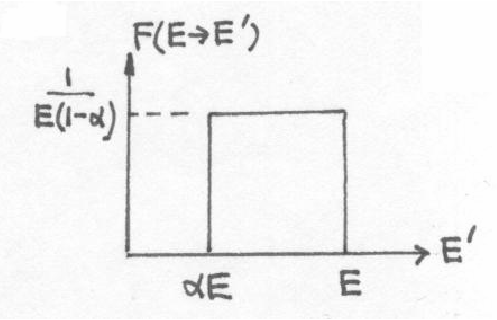
\includegraphics[width=2in]{images/ni/PT1toT3.png}
    \caption{Probability of Scattering from T1 to T3\label{PT1toT3}}
\end{figure}

We did not go into detailed calculation in class, but it is good to know that: elastic scattering cross section has a $\frac{1}{v}$ behavior at low energy (or high temperature), and a constant behavior at high energy. 


\end{document}
